
%%%%%%%%%%%%%%%%%%%%%%%%%%%%%%%%%%%%%%%%%%%%%%%%%%%%%%%%%%%%%%%%%%%%%
%% This is a (brief) model paper using the achemso class
%% The document class accepts keyval options, which should include
%% the target journal and optionally the manuscript type.
%%%%%%%%%%%%%%%%%%%%%%%%%%%%%%%%%%%%%%%%%%%%%%%%%%%%%%%%%%%%%%%%%%%%%
\documentclass[journal=jacsat,manuscript=article]{achemso}

%%%%%%%%%%%%%%%%%%%%%%%%%%%%%%%%%%%%%%%%%%%%%%%%%%%%%%%%%%%%%%%%%%%%%
%% Place any additional packages needed here.  Only include packages
%% which are essential, to avoid problems later. Do NOT use any
%% packages which require e-TeX (for example etoolbox): the e-TeX
%% extensions are not currently available on the ACS conversion
%% servers.
%%%%%%%%%%%%%%%%%%%%%%%%%%%%%%%%%%%%%%%%%%%%%%%%%%%%%%%%%%%%%%%%%%%%%
\usepackage[version=3]{mhchem} % Formula subscripts using \ce{}
\usepackage{amsmath}
\usepackage{xcolor}
\usepackage{amsfonts}
\usepackage{amssymb}
\usepackage{graphicx}
\usepackage[english]{babel}
\usepackage{chemfig}
\newcommand{\species}[1]{\textit{#1} sp.}
\usepackage{subcaption}
\usepackage{cancel}




%%%%%%%%%%%%%%%%%%%%%%%%%%%%%%%%%%%%%%%%%%%%%%%%%%%%%%%%%%%%%%%%%%%%%
%% If issues arise when submitting your manuscript, you may want to
%% un-comment the next line.  This provides information on the
%% version of every file you have used.
%%%%%%%%%%%%%%%%%%%%%%%%%%%%%%%%%%%%%%%%%%%%%%%%%%%%%%%%%%%%%%%%%%%%%
%%\listfiles

%%%%%%%%%%%%%%%%%%%%%%%%%%%%%%%%%%%%%%%%%%%%%%%%%%%%%%%%%%%%%%%%%%%%%
%% Place any additional macros here.  Please use \newcommand* where
%% possible, and avoid layout-changing macros (which are not used
%% when typesetting).
%%%%%%%%%%%%%%%%%%%%%%%%%%%%%%%%%%%%%%%%%%%%%%%%%%%%%%%%%%%%%%%%%%%%%
\newcommand*\mycommand[1]{\texttt{\emph{#1}}}

%%%%%%%%%%%%%%%%%%%%%%%%%%%%%%%%%%%%%%%%%%%%%%%%%%%%%%%%%%%%%%%%%%%%%
%% Meta-data block
%% ---------------
%% Each author should be given as a separate \author command.
%%
%% Corresponding authors should have an e-mail given after the author
%% name as an \email command. Phone and fax numbers can be given
%% using \phone and \fax, respectively; this information is optional.
%%
%% The affiliation of authors is given after the authors; each
%% \affiliation command applies to all preceding authors not already
%% assigned an affiliation.
%%
%% The affiliation takes an option argument for the short name.  This
%% will typically be something like "University of Somewhere".
%%
%% The \altaffiliation macro should be used for new address, etc.
%% On the other hand, \alsoaffiliation is used on a per author basis
%% when authors are associated with multiple institutions.
%%%%%%%%%%%%%%%%%%%%%%%%%%%%%%%%%%%%%%%%%%%%%%%%%%%%%%%%%%%%%%%%%%%%%

\author{Sperydon Koumarianos}
\affiliation{Department of Physics and Astronomy, York University, Toronto, ON, Canada. M3J 1P3} 
\alsoaffiliation{Department of Mathematics, York University, Toronto, ON, Canada.  M3J 1P3}

 
\author{Rohith Kaiyum}
\affiliation{Department of Physics and Astronomy, York University, Toronto, ON, Canada. M3J 1P3} 

\author{Christopher J. Barrett}
\affiliation{Department of Chemistry, McGill University, Montreal, QC, Canada.  H3A 2K6}

\author{Neal Madras}
\affiliation{Department of Mathematics, York University, Toronto, ON, Canada.  M3J 1P3}

\author{Ozzy Mermut}
\affiliation{Department of Physics and Astronomy, York University, Toronto, ON, Canada. M3J 1P3}
\email{omermut@yorku.ca}



\title[An \textsf{achemso} demo]
  {Effect of Chain Length on the Layered Adsorption of Polyelectrolytes to Surfaces: Supplement}


\keywords{American Chemical Society, \LaTeX}

\begin{document}
\subsection{1. Derivation of Mean-field lattice model}

\subsubsection{1.1 Setup of Mean-field lattice model}

We shall use a lattice model to describe our experimental situation.  
Lattices will appear in two ways:  (1) covering the surface of a sphere by a two-dimensional lattice, and
(2) filling space with a regular three-dimensional lattice.  
The geometry of the lattices will not be important.  We shall use the simple cubic lattice for our
three-dimensional lattice.  
We shall assume that the two-dimensional lattice has coordination number $q$ 
(that is, each site on the surface has exactly $q$ neighbouring sites).  We assume that 
the distance between lattice sites corresponds to the distance between adjacent monomers within a 
polymer.  We assume that in equilibrium, \textit{every lattice site in the surface is covered by an adsorbed 
monomer}.

Our experiment has a large number $n_{sphere}$ of spheres in a solution of volume $V_{sol}$.  To simplify 
our model and keep the concentrations the same, we shall consider only a single sphere in a solution
of volume $V_1:=V_{sol}/n_{sphere}$.  We shall refer to this as our model system.
We shall view this small three-dimensional region of the solution in our model system as being filled by a 
cubic lattice.
Let $V_{latt}$ be the number of lattice sites in our solution region of volume $V_1$. This is illustrated in the simple graphic in Figure 1.

%fix to make more sense with above, flow
% More specifically, in Figure 1 we illustrate the total solution volume, and a subdivision of it on the order of 0.01\%. The goal of this was to subdivide the total solution volume into "micro-volumes" that each occupy one colloid and an $n_S$ quantity of short chain polymers ($PAA_{2k}$) and $n_L$ quantity of long chain polymers ($PAA_{450k}$). This was acheived by initially approximating the quantity of colloids, this was done by letting the solution be contained in a standard laboratory beaker of volume 0.5L. The total number of colloids in 0.5L of solution was calculated to be approximately 1300 colloids which would imply that one colloid corresponds to 0.07\% of the total number colloids in a 0.5L beaker of solution. The total volume of solution was then subdivided into 1300 equally sized micro-volumes, of approximately $3.77 x 10^{-4}L$. We focused our modelling and calculations on those very microvolume assuming that the distribution of particles in solution are approximately uniform, and that the behaviours seen in one subdivision of solution can be generalized to the whole solution, given that the whole system is solely entropy driven.


\begin{figure}[H] 
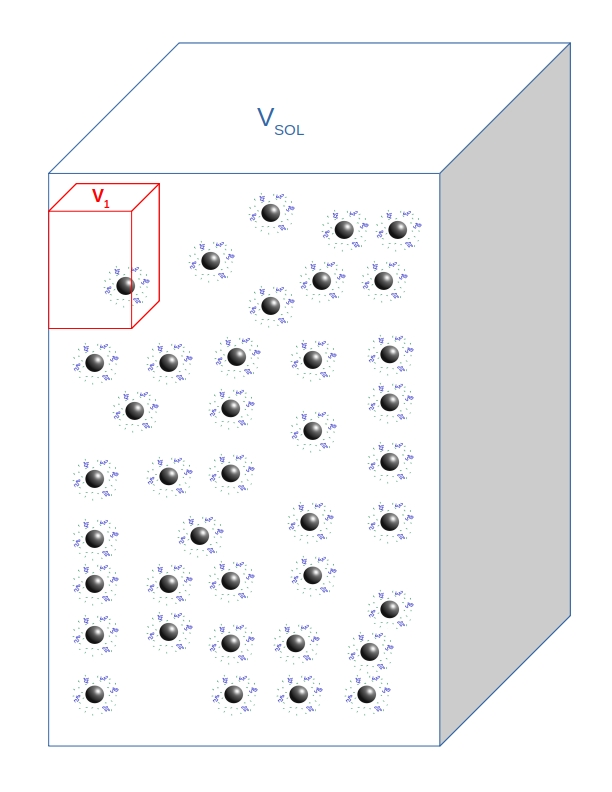
\includegraphics[scale=0.5]{fig7.jpg}
\caption{}
\label{figure 7}
\end{figure}

\subsubsection{1.2 Explaining "Step by Step" Model}

We shall consider polymers of two different lengths, which we shall call ``short'' and ``long.''  Their lengths
will be described by two positive integer parameters $W$ and $n$.

\begin{verse}
A \textbf{short polymer} will consist of $W$ monomers.  
Let $n_S$ be the number of short polymers in the model system. 
\\
A \textbf{long polymer} will consist of $nW$ monomers.  
Let $n_L$ be the number of long polymers in the model system. 
\end{verse}
We shall often refer to our short and long polymers as $W$-mers and $nW$-mers respectively.
We shall want the total mass of the two kinds of monomers in our system to be the same, so we 
shall assume that $n_S \,=\, n\cdot n_L$.

Let $A_{latt}$ be the number of lattice sites on the surface of one sphere, and let $a$
be the number of long polymers that would exactly cover all the sites of the surface:
\[    a  \;=\;  \frac{A_{latt}}{nW}   \,  .  \]
Then $na$ is the number of short polymers that can completely cover the surface.
For simplicity, we assume that $a$ is an integer.

We shall see that the underlying entropic reason that
mostly long chains get adsorbed is that $V_{latt}\gg A_{latt}$, i.e.\ there are many more possible locations in 
the three-dimensional solution than on the two-dimensional surface.


We shall model our polymer configurations in the solution in a slightly different way from those on the surface.
The difference in approach is due to the fact that the polymers are dense on the surface but 
dilute in the solution.  We shall model the polymer configurations in the solution as a collection of 
self-avoiding walks in the cubic lattice, with no interaction between walks (because of the dilute solution).
For the polymers adsorbed densely on the surface lattice, we shall use mean-field calculations 
of the Flory-Huggins type 
% (similar to the lattice approach in Park et al., Macromolecules 2001;
(see also Section XII.1 of \cite{Flory1953}).

Recall that our ensemble consists of $n_S$ (short) $W$-mers and $n_L$ (long) $nW$-mers.
Of these, some are adsorbed onto the surface of the sphere, and the others float freely in the 
solution of volume $V_1$.  We write $j$ for the number of (long) $nW$-mers that are adsorbed 
onto the surface in a particular configuration of the system.  This implies that
\begin{verse}
 ($i$) the number of $nW$-mers in solution is $n_L-j$;
 \\
 ($ii$) the number of $W$-mers adsorbed on the surface is $n(a-j)$ (because there are $anW$ sites on the
 surface, all occupied, of which $jnW$ are occupied by $nW$-mers, leaving $anW-jnW$ to be 
 occupied by $W$-mers); and
 \\
 ($iii$) the number of $W$-mers in solution is $n_S-n(a-j)$.
 \end{verse}  
We shall write $\mathcal{E}_j$ for the set of all configurations that have exactly $j$ $nW$-mers adsorbed 
onto the surface.  Observe that the possible values of $j$ are the integers from 0 to $a$.
The full space of configurations in our model is $\cup_{j=0}^a {\mathcal{E}_j}$, 
which we shall call $\mathcal{E}$.

Since the only energy in this model comes from the adsorption contacts between monomer and surface,
and since the number of such contacts is the same (namely $A_{latt}$) in every configuration
in $\mathcal{E}$, we see that the energy of every configuration of $\mathcal{E}$ is exactly the same.
Therefore, according to the Boltzmann distribution, \textit{every configuration in $\mathcal{E}$ is equally
likely}.  Thus the calculation of probabilities of events is equivalent to counting the configurations.
In particular, writing $|\mathcal{A}|$ for the number of configurations in a set $\mathcal{A}$, we have
\[
    \hbox{Probability that $j$ long polymers are adsorbed}  \;=\; 
    \frac{|\mathcal{E}_j|}{|\mathcal{E}|}\,,   \hspace{5mm}(j=0,1,\ldots,a).
\]
Thus, to find the most likely number of $nW$-mers (and $W$-mers) to be adsorbed onto the sphere,
we need to find which of the sets $\mathcal{E}_j$ is largest.

In order to better comprehend the model we provide an illustration figure 6.8 with much simpler values than what would be considered the standard chain lengths in polymer science. We let each lattice point of area of one mer of PAA, be a square on the grid. Additionally, each long chain mer contact is represented by an L and a Short Chain mer by an S on the grid.  Suppose a short chain is 30-mers and long chain is 90-mers and the colloid surface has 3000 available single mer sites. The model is initialized with the colloid surface sites absolutely covered in exclusively short chains  which in this concrete example is 100 short chains. We then remove enough short chains in order to be able to replace them with our first long which in this example is occupies the sites of 3  short chains. We will continue to do this successive combination sampling process of adding more and more Long chains in place of the equivalent number of mers in short chains until we get a maximal value for $\mathcal{E}_{j}$.

\begin{figure}[H]
    \begin{subfigure}[b]{0.4\textwidth}
        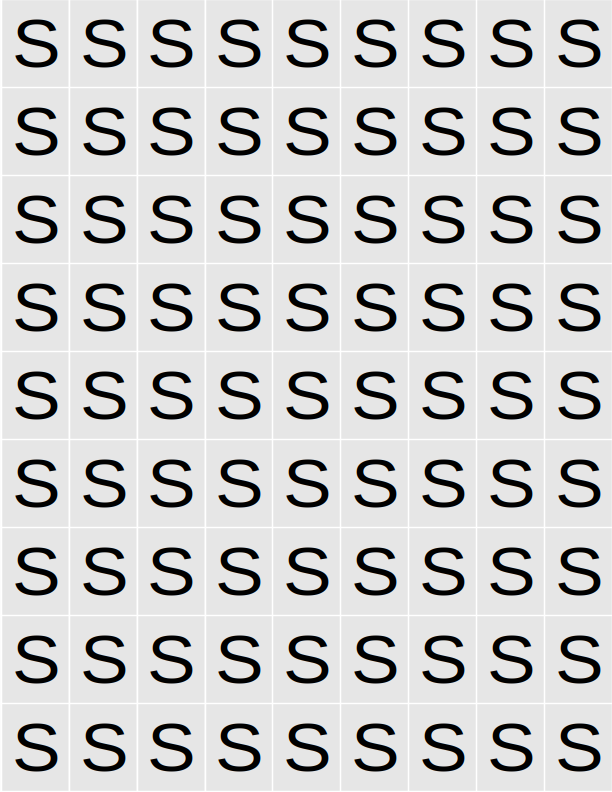
\includegraphics[scale=0.15]{fig8a.png}
        \caption{0 Long \& 81 Short chains\\ on Colloid Surface}
        \label{fig:A}
    \end{subfigure}
    \begin{subfigure}[b]{0.4\textwidth}
        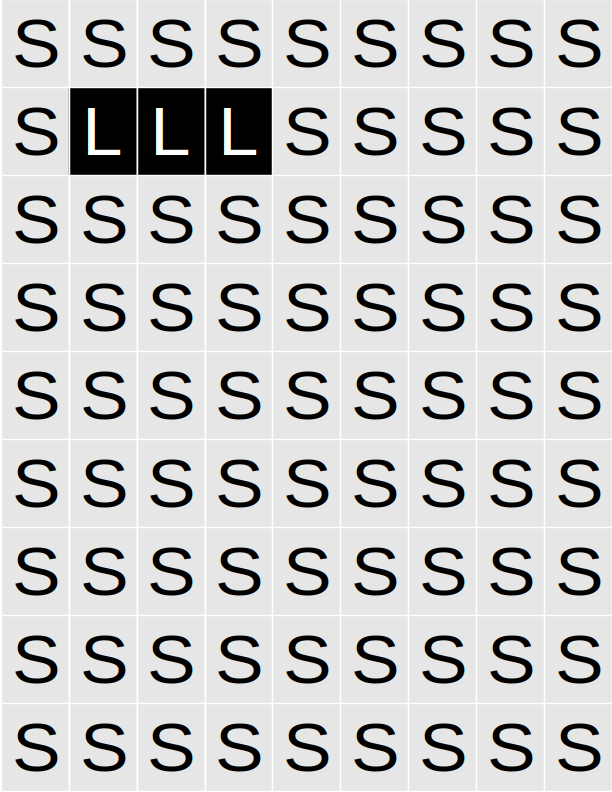
\includegraphics[scale=0.15]{fig8b.png}
        \caption{1 Long \& 78 Short chains\\ on Colloid Surface}
        \label{fig:B}
    \end{subfigure}
    %\textbf{}\\
    \begin{subfigure}[b]{0.4\textwidth}
        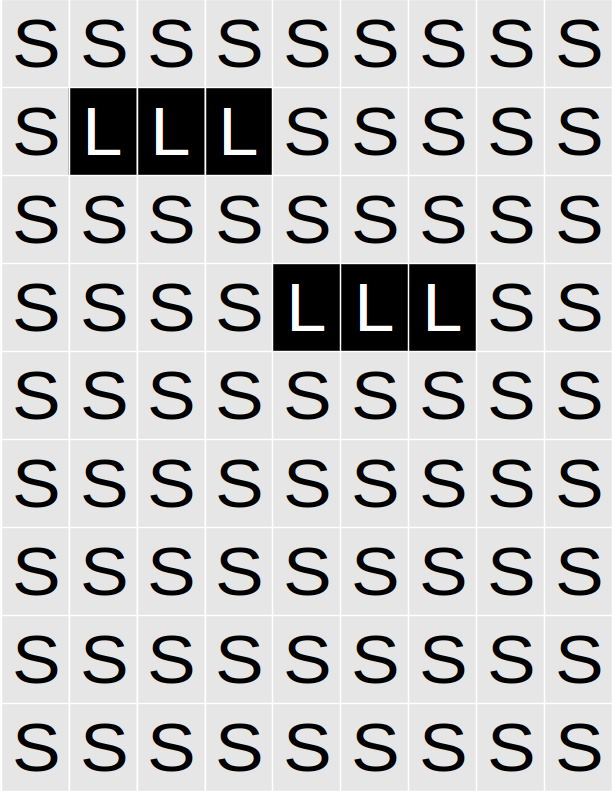
\includegraphics[scale=0.15]{fig8c.png}
        \caption{2 Long \& 75 Short Chains\\ on Colloid Surface}
        \label{fig:C}
    \end{subfigure}
    \begin{subfigure}[b]{0.4\textwidth}
        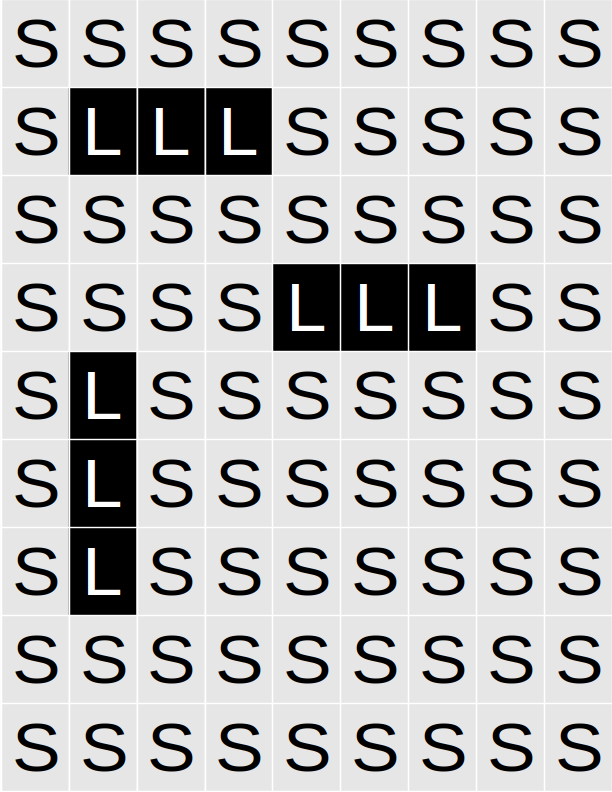
\includegraphics[scale=0.15]{fig8d.png}
        \caption{3 Long \& 72 Short Chains\\ on Colloid Surface}
        \label{fig:D}
    \end{subfigure}
    \begin{subfigure}[b]{0.4\textwidth}
        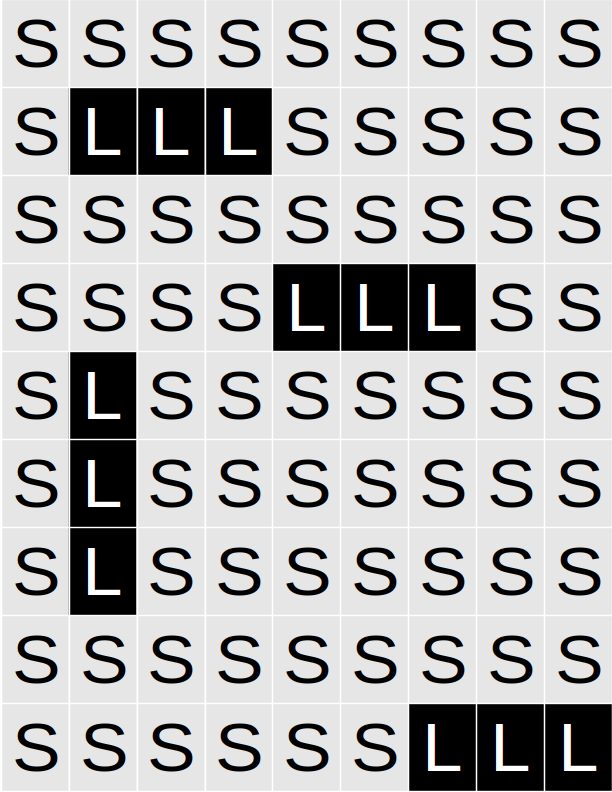
\includegraphics[scale=0.15]{fig8e.png}
        \caption{4 Long \& 69 Short Chains\\ on Colloid Surface}
        \label{fig:E}
    \end{subfigure}
    \begin{subfigure}[b]{0.4\textwidth}
        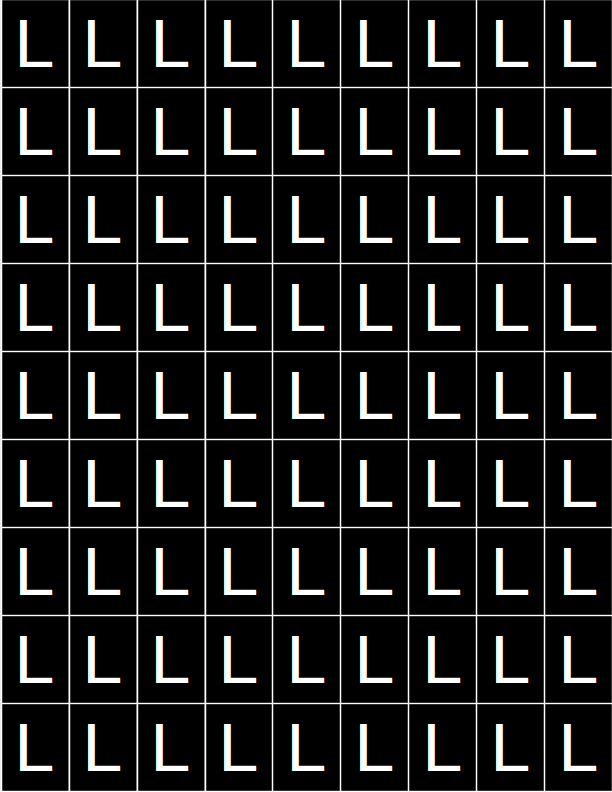
\includegraphics[scale=0.15]{fig8f.png}
        \caption{27 Long \& 0 Short Chains\\ on Colloid Surface}
        \label{fig:F}
    \end{subfigure}
    \caption{Process of Sampling Full Surface Coverage Combinations of ever increasing Long Chains that are substituting multiple Short Chains  on Colloid}
\end{figure}

\noindent We now proceed to estimate the size of each $\mathcal{E}_j$.

\smallskip

The configuration of a single  polymer in a dilute solution is often modeled by
a self-avoiding walk (SAW) in a lattice, i.e.\  a path in the lattice that does not visit any site more than once.
A fundamental property of SAWs is the following.  
Let $c_{\ell}$ be
the number of SAWs that start from a specified lattice site (``the origin'') and visit a total of $\ell$ sites
(including the starting site).   Then the 
asymptotic behaviour of $c_{\ell}$ on the three-dimensional cubic lattice is 
\begin{equation}
    \label{eq.sawscale}
       c_{\ell}  \;\sim  \;  A_3 \, {\ell}^{\gamma_3-1}  \mu_3^{\ell}    \hspace{5mm}\hbox{as $\ell\rightarrow\infty$}.
\end{equation}
% (This has not been proven rigorously, but even mathematicians do not doubt its truth.) 
Here $\mu_3$ and $A_3$ depend on the choice of lattice, but $\gamma_3$ is a universal critical exponent
that is the same for all three-dimensional lattices.  
Their values are known to be approximately \cite{Chen2002,Madras2013}
\begin{equation}
   \label{eq.gammas}   \mu_3 \;=\;  4.684, \hspace{5mm}
        \gamma_3 \;=\;  1.162,    \hspace{5mm}\hbox{and}\hspace{5mm}
    A_3  \;=\;    0.2573  \,.  %1.205/4.683 \;=\;  \,.
\end{equation}
(Estimation in \cite{Chen2002} is for the 
number of SAWs with $\ell$ \textit{steps} (i.e.\ $\ell+1$ \textit{sites}), which we write  $c_{\ell+1}=(A_3\mu_3)\ell^{\gamma_3-1}\mu_3^{\ell}$; reference \cite{Chen2002} obtains $A_3\mu_3=1.205$.)

Since the number of sites in the lattice corresponding to the region of solution is $V_{latt}$, 
we have $V_{latt}c_{\ell}$ ways to place a polymer of size ${\ell}$.  As we are neglecting the
possibility of overlapping polymers in the dilute solution, it follows that the number of ways to 
place $N$ identical $\ell$-mers is 
\begin{equation}
  \label{eq.Npoly}
   \frac{(V_{latt}c_{\ell})^N}{N!}  \,.   
\end{equation}

\smallskip

For a particular choice of $j$, we want to know the number of ways to place $j$ $nW$-mers 
and $a(n-j)$ $W$-mers on the surface, without overlapping, to fill all $anW$ lattice sites on the surface.
This is a hard combinatorial problem, so we shall use the following mean-field (Flory-Huggins) approach.
We shall place one polymer at a time, starting with the long ones.
Let $\tilde{w}_k$ be the number of ways to place the $k^{th}$ $nW$-mer on the surface, given that
$(k-1)$ $nW$-mers have already been placed.  
To begin with, there are $anW-(k-1)nW$ available sites for the first monomer.  Recall that  $q$ is the number of
neighbours of each site in the surface lattice.
In the absence of other polymers, there would be $q$ choices for the second monomer in the chain,
and $q-1$ choices for each monomer after that (here we are using the non-reversed walk model of a polymer
instead of the fully self-avoiding model).  But the number of choices should on average be reduced 
by the fraction of the surface that has already been covered.  
Thus, when we are trying to place the second monomer of our chain, there are
$anW-(k-1)nW-1$ unoccupied sites, so each site has 
probability $[anW-(k-1)nW-1]/[anW]$ of being available.  
Thus there are $q[anW-(k-1)nW-1]/[anW]$ choices for the second monomer.  
Similarly, after $i$ monomers of the current chain have been placed ($i\geq 2$), the fraction of the
surface that has been covered is $[anW-(k-1)nW-i]/[anW]$, so there are 
$(q-1)[anW-(k-1)nW-i]/[anW]$ choices for the $(i+1)^{th}$ monomer in this chain.  
We conclude that 
\begin{eqnarray}
   \tilde{w}_k  & = &   [anW-(k-1)nW]\,\times \,q\left(\frac{ anW-(k-1)nW-1}{anW}\right)    \,\times
   \nonumber    \\
   & &    \hspace{22mm}
     \prod_{i=2}^{nW-1}(q-1)\left(\frac{ anW-(k-1)nW-i}{anW}\right)  
      \nonumber \\
 & = &    \frac{[anW-(k-1)nW]!}{[anW-knW]!} \,q\,  \frac{(q-1)^{nW-2}}{(anW)^{nW-1}}  
     \nonumber    \\
     & = &    \frac{[anW-(k-1)nW]!}{[anW-knW]!}   anW \frac{q}{(q-1)^2}\left(  \frac{q-1}{anW}\right)^{nW}.
     \label{eq.wk2}
\end{eqnarray}
Similarly, let $\tilde{u}_{\ell}$ be the number of ways to place the $\ell^{th}$ $W$-mer on the surface, given that
${\ell}-1$ $W$-mers (or a total of $(\ell-1)W$ monomers) have already been placed.   The same 
argument as for $\tilde{w}_k$ gives
\begin{eqnarray}
   \tilde{u}_{\ell}  
 & = &    \frac{[anW-(\ell-1)W]!}{[anW-\ell W]!} \,q\,  \frac{(q-1)^{W-2}}{(anW)^{W-1}}  
     \nonumber    \\
     & = &    \frac{[anW-(\ell-1)W]!}{[anW-\ell W]!}   anW \frac{q}{(q-1)^2}\left(  \frac{q-1}{anW}\right)^{W}.
     \label{eq.uell2}
\end{eqnarray}

To evaluate $|\mathcal{E}_j|$, we assume that the unadsorbed solution
is dilute enough that we don't need to worry about mutual exclusion between the free floating
polymers.   
For $\mathcal{E}_j$, we have $j$ adsorbed $nW$-mers, $na-nj$ adsorbed $W$-mers, 
$n_L-j$ desorbed $nW$-mers, and $n_S-n(a-j)$ desorbed $W$-mers.   Thus, recalling 
Equations (\ref{eq.sawscale}) and  (\ref{eq.Npoly}), we have
\begin{equation}
    |\mathcal{E}_j|  
      \; = \; \frac{ \Psi_L^{n_L-j} }{(n_L-j)!} \,
          \frac{ \Psi_S^{n_S-n(a-j)} }{(n_S-n(a-j))!} \,
           \frac{\tilde{w}_1\tilde{w}_2\cdots \tilde{w}_j}{j!}
                     \,   \frac{\tilde{u}_{nj+1}\tilde{u}_{nj+2}\cdots \tilde{u}_{an}}{(n(a-j))!}
%                                  \nonumber   \\
%            & & \hspace{7mm}  \times \, \frac{\tilde{w}_1\tilde{w}_2\cdots \tilde{w}_j}{j!}
%                     \,   \frac{\tilde{u}_{nj+1}\tilde{u}_{nj+2}\cdots \tilde{u}_{an}}{(n(a-j))!}  % \,e^{-nW\epsilon/kT}
        \label{eq.Yj}
\end{equation}
where 
\begin{equation}
    \label{eq.psidef}   
   \Psi_L\;=\;V_{latt} A_3 (nW)^{\gamma_3-1} \mu_{3}^{nW}   
    \hspace{5mm}\hbox{and} \hspace{5mm}
     \Psi_S \;=\; V_{latt}A_3W^{\gamma_3-1}\mu_3^W \,.
\end{equation}




To determine which value of $j$ maximizes $|\mathcal{E}_j|$, we look at ratios of consecutive terms:
\begin{eqnarray}
    \frac{|\mathcal{E}_{j+1}|}{|\mathcal{E}_j|}   & = & 
 \frac{
     \left(\frac{\Psi_L^{n_{L}-j-1}}{(n_L-j-1)!}\right)\cdot\left(\frac{\Psi_S^{n_S-n(a-j-1)}}{
    (n_S-n(a-j-1))!}\right) 
      }{
 \left(\frac{\Psi_L^{n_{L}-j}}{(n_L-j)!}\right)\cdot\left(\frac{\Psi_S^{n_S-n(a-j)}}{
    (n_S-n(a-j))!}\right)  }  \,   \frac{\tilde{w}_{j+1} }{  \tilde{u}_{nj+1}\cdots \tilde{u}_{n(j+1)} } 
    \nonumber \\
    & & \hspace{42mm}  
     \times   \, \frac{ j! \, (na-nj)!}{(j+1)!\, (na-nj-n)!}  
    \nonumber    \\
    & = & \frac{\Psi_S^n}{\Psi_L}
   % \frac{ \left(  V_{latt} A_3 W^{\gamma_3-1}\right)^{n-1}}{n^{\gamma_3-1}}
    \,   \frac{\tilde{w}_{j+1} }{  \tilde{u}_{nj+1}\cdots \tilde{u}_{n(j+1)} }   \,\left(  \frac{n_L-j}{j+1}\right)
    \nonumber \\
    & &   \hspace{8mm}  \times \;  \frac{(na-nj)\cdots (na-nj-n+1)}{(n_S-na+nj+1)\cdots(n_S-na+nj+n)} \,.
        \label{eq.Yratio1}
\end{eqnarray}
By Equation (\ref{eq.psidef}), we have
\begin{equation}
   \label{eq.psiratio} 
      \frac{\Psi_S^n}{\Psi_L}   \;=\;   \frac{ (V_{latt}\, A_3 \,W^{\gamma_3-1})^{n-1}}{n^{\gamma_3-1}}\,.
\end{equation}
From Equations (\ref{eq.wk2}) and (\ref{eq.uell2}), we find
\begin{eqnarray}
     \frac{\tilde{w}_{j+1} }{  \tilde{u}_{nj+1}\cdots \tilde{u}_{n(j+1)} }  & = & 
        \left( \frac{(q-1)^2}{qanW}\right)^{n-1}   \times \,
    \frac{   \frac{(anW-jnW)!}{(anW-(j+1)nW)!}  }{
        \prod_{\ell=0}^{n-1} \frac{ (anW-(nj+\ell)W)!}{(anW-(nj+\ell+1)W)!}   }
     \nonumber  \\
     & = & \left( \frac{(q-1)^2}{qanW}\right)^{n-1}  \,\times\, 1.
     \label{eq.Yratioa}     
\end{eqnarray}
Next we use the approximation   $(a+1)(a+2)\cdots (a+m-1) \,\approx \,(a+\frac{m}{2})^m$
(essentially, replacing the geometric mean by the arithmetic mean) to obtain
\begin{equation}
       \frac{(na-nj)\cdots (na-nj-n+1)}{(n_S-na+nj+1)\cdots(n_S-na+nj+n)} 
       \; \approx \;    \frac{ [na-(j+\frac{1}{2})n]^n }{ [n_S-na+nj+\frac{n}{2}]^n} \,.\hspace{3mm}
  %     \nonumber  \\
  %     & \approx & \left(  \frac{n(a-j-\frac{1}{2})}{n_S-(a-j-\frac{1}{2})}\right)^n  .
      \label{eq.Yratiob}
\end{equation} 
Now, putting Equations (\ref{eq.psiratio}--\ref{eq.Yratiob}) back into (\ref{eq.Yratio1}), we obtain
\begin{equation}
    \label{eq.Yratio2}
       \frac{|\mathcal{E}_{j+1}|}{|\mathcal{E}_j|} \; \approx \; 
       \left(  \frac{ V_{latt}A_3W^{\gamma_3-1}(q-1)^2}{aWq} \,
          \frac{(a-j-\frac{1}{2})}{n_S-n(a-j-\frac{1}{2})} \right)^{n+o(n)}   \,.
\end{equation}
The quantity on the right of Equation (\ref{eq.Yratio2}) decreases in $j$.  Let $j^*$ be the 
smallest value of $j$ for which the right-hand side of Equation (\ref{eq.Yratio2}) is less than 1.
Then we see that $|\mathcal{E}_{j+1}|/|\mathcal{E}_j|<1$ whenever $j\geq j^*$, and 
$|\mathcal{E}_{j+1}|/|\mathcal{E}_j|\geq 1$ whenever $j< j^*$.
That is, $|\mathcal{E}_j|$ is decreasing in $j$ when $j\geq j^*$, and 
increasing when $j< j^*$.
It follows that $|\mathcal{E}_j|$ is maximized at $j=j^*$, and that we can find $j^*$ by seeing 
where the right-hand side of Equation (\ref{eq.Yratio2}) is close to 1.   Thus $j^*$ satisfies
\[     1  \;\approx \; 
     K  \,%\frac{ V_{latt}A_3W^{\gamma_3-1}(q-1)^2}{aWq} \,
          \frac{a-j^*-\frac{1}{2}}{n_S-n(a-j^*-\frac{1}{2})}    \,,  
             \hspace{5mm}\hbox{where}\hspace{5mm}
             K \;=\;   \frac{ V_{latt} }{aW}\, \frac{   A_3W^{\gamma_3-1}(q-1)^2}{q} \,,
\]
which can be rewritten as 
\[       a-j^*-\frac{1}{2} \; \approx\;    \frac{n_S}{K+n}   \,.
\]
We observe that $K\gg n$; indeed,  $V_{latt}/aWn \,=\,V_{latt}/A_{latt}\gg 1$.  
Thus we can replace $K+n$ by $K$ in the above, and omit the term $\frac{1}{2}$, resulting in the   
approximation 
\begin{equation}
    \label{eq.jstar}
     1-\frac{j^*}{a}     \; \approx   \; 
        \left(  \frac{n_S\,W}{V_{latt} }\right) \,\left(   \frac{q}{A_3W^{\gamma_3-1}(q-1)^2}\right)  \,.
\end{equation}
The above equation can be interpreted as follows.  The left hand side, $1-j^*/a$, is the fraction of the
sphere's surface that is covered by short monomers.  The ratio $n_SW/V_{latt}$ gives
the concentration of monomers corresponding to those appearing on the short chains only.
The quantity in the second set of 
parentheses in Equation (\ref{eq.jstar}) cannot be large, since $q<(q-1)^2$ and $\gamma_3>1$.
If the solution is fairly dilute, then we see that the left side of (\ref{eq.jstar}) is small,
and hence only a small fraction of the surface is covered by short polymers.


[\textit{Remark:}  Observe that $n_L$ does not appear in Equation (\ref{eq.jstar}).  
In the expression for $|\mathcal{E}_{j+1}|/|\mathcal{E}_j|$,   only $n_S$ appears inside the 
expression that is raised to the power $n$, while $n_L$ appears outside this expression and is
raised to the power 1.]  

\section{Interpretations about $\mathcal{E}_{j}$ from ratio $\frac{\mathcal{E}_{j+1}}{\mathcal{E}_{j}}$}

What is graphically portrayed in Figure 9, is that as one increases the number of long chains in a scenario of full surface coverage of the colloid, the ratio of probabilities crosses the threshold of the functional value being equal to one ($\frac{\mathcal{E}_{j+1}}{\mathcal{E}_{j}}=1$), this threshhold is representative of two consecutive configurations being equal in value and thus the the divided differences of $\mathcal{E}_{j+1}$ and $\mathcal{E}_{j}$ being equal to zero for interval,  $j\in[j^*, j^*+1]$. This preceeding statement is suggestive of the existence of a maximal critical point. 

%needs a zero on the corner
\begin{figure}[H]
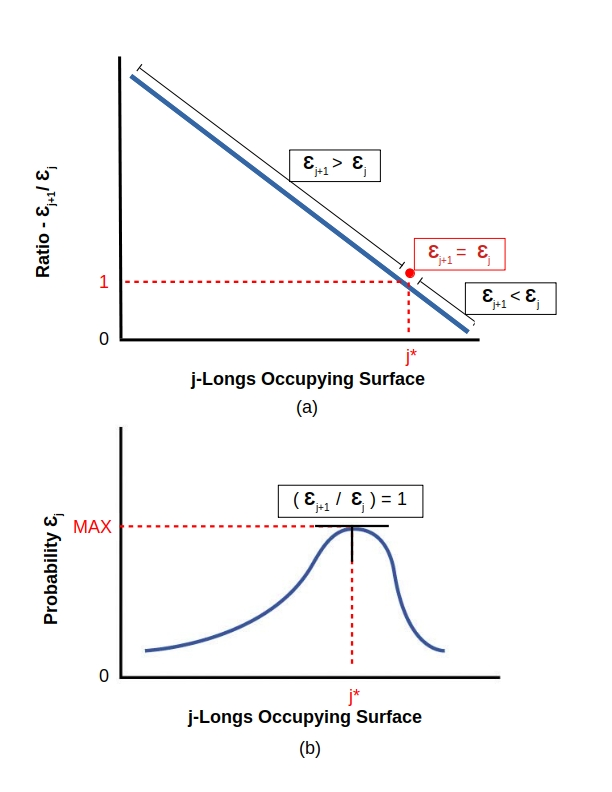
\includegraphics[scale=0.50]{fig9ab.jpg}
\caption{}
\label{figure 9}
\end{figure}

\subsubsection{1.3 Derivation of Boltzmann Entropy from Ratio Approximation}

Intially, we shall take the natural logarithm of our ratio $\frac{\mathcal{E}_{j+1}}{\mathcal{E}_{j}}$. Then we proceed to expand the expression using known logarithmic properties and multiply the whole expression by the Boltzmann Constant.
$$log\left(\frac{\mathcal{E}_{j+1}}{\mathcal{E}_{j}}\right)$$
$$=k_B\cdot\left(log\left(\mathcal{E}_{j+1}\right)\right)-\left(log\left(\mathcal{E}_{j}\right)\right)$$
$$= \left(k_B\cdot log\left(\mathcal{E}_{j+1}\right)\right)-\left(k_B\cdot log\left(\mathcal{E}_{j}\right)\right)$$

\noindent this is evidently, just the difference of Boltzman entropies of j and j+1,

$$=S_{j+1}-S_{j}=\Delta S_{j\to j+1}$$

\section{One-dimensional model}

We now present a more tractable ``toy'' version of the lattice model.  We shall assume that 
the surface is one-dimensional, which eliminates the need for the Flory-Huggins-type approximations.

As before, we have $n_S$ short $W$-mers and $n_L$ long $nW$-mers, some of which are adsorbed 
onto a surface with $anW$ lattice sites, and the rest float as free self-avoiding walks 
in a three-dimensional cubic lattice with  $V_{latt}$ sites.  
The difference now is that we shall replace the spherical surface with a line segment
$\mathcal{S}$ containing $anW$ sites.  When a short (respectively, long) polymer is adsorbed, it covers a 
sub-segment of $\mathcal{S}$ containing $W$ (respectively, $nW$) sites.
If exactly $j$ long polymers are adsorbed onto $\mathcal{S}$, then $n(a-j)$ short polymers are
also adsorbed.  The number of ways that this can be done depends only on the order in which 
longs and shorts appear when traversing $\mathcal{S}$ from one end to the other.  Since the total 
number of adsorbed polymers in this case is $n(a-j)+j$, the number of ways is 
\[      \binom{n(a-j)+j}{j}   \,.  \]
As before, let $\mathcal{E}_j$ be the number of ways to place $j$ $nW$-mers and $a(n-j)$ $W$-mers on 
$\mathcal{S}$, as well as $n_L-j$ $nW$-mers and $n_S-a(n-j)$ $W$-mers as self-avoiding walks 
in the three dimensional lattice.  Then we have 
\begin{equation}
   \label{eq.1dE}
    |\mathcal{E}_j| \;=\;  \left(\frac{\Psi_L^{n_{L}-j}}{(n_L-j)!}\right)\cdot\left(\frac{\Psi_S^{n_S-n(a-j)}}{
    (n_S-n(a-j))!}\right) \cdot\binom{an-jn+j}{j}   \,,
\end{equation}
where 
$\Psi_L$ and $\Psi_S$ are as defined in Equation (\ref{eq.psidef}).
%\[       \Psi_L\;=\;V_{latt} A_3 (nW)^{\gamma_3-1} \mu_{3}^{nW}   
%    \hspace{5mm}\hbox{and} \hspace{5mm}
%     \Psi_S \;=\; V_{latt}A_3W^{\gamma_3-1}\mu_3^W \,.    \]

We shall show that for the one-dimensional model, $|\mathcal{E}_j|$ increases rapidly as $j$ increases,
and hence the likeliest situation is complete coverage by long polymers.  To do this, we shall show that
$|\mathcal{E}_{j+1}|/|\mathcal{E}_j| \,\gg\,1$ for every $j=0,\ldots,a-1$.

From Equation (\ref{eq.1dE}), we have
\begin{align}
   \nonumber
    \frac{|\mathcal{E}_{j+1}|}{|\mathcal{E}_j|} \; & =\;   
    \frac{
     \left(\frac{\Psi_L^{n_{L}-j-1}}{(n_L-j-1)!}\right)\cdot\left(\frac{\Psi_S^{n_S-n(a-j-1)}}{
    (n_S-n(a-j-1))!}\right) \cdot\left( \frac{ (an-jn-n+j+1)!}{(j+1)!(an-jn-n)!} \right)
      }{
 \left(\frac{\Psi_L^{n_{L}-j}}{(n_L-j)!}\right)\cdot\left(\frac{\Psi_S^{n_S-n(a-j)}}{
    (n_S-n(a-j))!}\right) \cdot   \left( \frac{ (an-jn+j)!}{j!(an-jn)!} \right)    }
    \\
    \nonumber
    & = \;   \left( \frac{\Psi_S^n \,(n_L-j) }{\Psi_L \, \prod_{k=1}^n[n_S-na+nj+k]  }\right)  \,\times 
     \\
     \nonumber
    & \hspace{31mm}  \left(   \frac{  \prod_{k=0}^{n-1}[an-jn-k]    }{(j+1)  \prod_{k=0}^{n-2} [an-jn+j-k]   }\right)
    \\
    \label{eq.1dEE}
      & \approx \;   \frac{ \Psi_S^n \,(n_L-j) [an-jn-\frac{n}{2}]^n
         }{   \Psi_L (j+1)  [n_S-na+nj+\frac{n}{2}]^n  [an-jn+j-\frac{n}{2}]^{n-1} }   \,.
\end{align}
Using Equation (\ref{eq.psiratio}) in 
 Equation (\ref{eq.1dEE}), we obtain 
\begin{equation}
   \label{eq.1dEEb}  
    \frac{|\mathcal{E}_{j+1}|}{|\mathcal{E}_j|} \; \approx  \;   
      \left(   \frac{ V_{latt}\, A_3 \,W^{\gamma_3-1} }{n_S-na+nj+\frac{n}{2}} \cdot 
         \frac{ an-nj-\frac{n}{2} }{an-jn-\frac{n}{2}+j}   \right)^{n+o(n)}.
\end{equation}
The first quotient inside the parentheses in Equation (\ref{eq.1dEEb}) is large:  indeed,
$V_{latt}/(n_S-na+nj)$ equals $W$ divided by the fraction of the solvent lattice that is occupied by 
short polymers.  
And the second quotient inside the parentheses is close to 1 for large $n$.   Therefore 
Equation (\ref{eq.1dEEb}) tells us that $|\mathcal{E}_{j+1}|/|\mathcal{E}_j| \,\gg\,1$
for every $j$.  It follows that configurations are highly likely to be in $\mathcal{E}_a$, i.e.\
to have $\mathcal{S}$ covered entirely by long polymers.
\bibliography{LongShort}
\end{document}